
\documentclass[border=3pt,tikz]{standalone}
\usetikzlibrary{calc}
\usetikzlibrary{fadings}




\begin{document}
	
	
% Author: Izaak Neutelings (June 2020)
% Inspiration:
%   https://www.researchgate.net/figure/a-Refractive-index-and-b-dispersion-of-bulky-soft-glasses-NC21-LLF1-SF6-and-F2-As_fig1_236110630
%   https://link.springer.com/article/10.1007/s11082-014-9979-y	
% DROPLET dispersion & rainbow
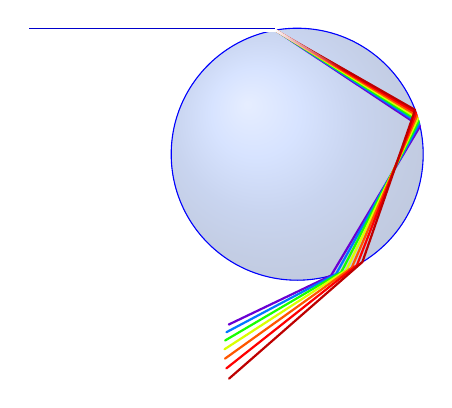
\begin{tikzpicture}
\colorlet{myblue}{blue!80!black}
\colorlet{myred}{black!50!red}
\colorlet{watercol}{blue!70!cyan!50}
\tikzstyle{myarr}=[-{Latex[length=3,width=2]}]
\tikzstyle{water}=[ball color=watercol]
\tikzset{
beam/.style={very thick,line cap=round,line join=round},
}		
\def\L{2.4}    % length of ray outside droplet
\def\R{1.8}    % droplet radius
\def\na{1.0}   % air
\def\nw{1.33}  % water
\def\alphI{150}                                   % A: incident (180-90)
\pgfmathsetmacro\thetI{180-\alphI}                % theta_1: incident
\pgfmathsetmacro\thetII{asin(\na/\nw*sin(\thetI)} % theta_2: air -> water & reflection
\pgfmathsetmacro\alphII{\alphI+2*\thetII-180}     % C: reflected
\pgfmathsetmacro\alphIII{\alphI+4*\thetII-360}    % D: exiting
\pgfmathsetmacro\py{\R*sin(\alphI)/sin(\alphII)}  % intersection height
\coordinate (O) at (0,0);
\coordinate (A) at (-\L-0.5*\R,{\R*sin(\alphI)});    % incident ray
\coordinate (B) at (\alphI:\R);                      % entry of incident
\coordinate (C) at (\alphII:\R);                     % internal reflection
\coordinate (D) at (\alphIII:\R);                    % exit of ray
\coordinate (E) at ($(D)+(\alphIII-\thetI:0.7*\L)$); % final ray to observer
\coordinate (P) at (\alphII:\py);                    % intersection point		
	
	
	\def\L{1.8}            % length of ray outside droplet
	\def\R{1.6}            % droplet radius
	\def\na{1.0}           % air
	\def\N{6}              % number of rays
	\def\alphI{100}        % A: incident (180-90)
	\pgfmathsetmacro\thetI{180-\alphI} % theta_1: incident
	
	% WATER DROPLET
	\fill[water] (O) circle (\R);
	\fill[watercol!20,opacity=0.8] (O) circle (\R);
	\draw[blue] (O) circle (\R);
	
	% LIGHT RAYS
	\coordinate (O) at (0,0);
	\coordinate (A) at (-\L-\R,{\R*sin(\alphI)}); % incident ray
	\foreach \i [evaluate={
		\lamb=410+\i*320/\N;              % wavelength (for color)
		\nw=1.36-0.08*\i/\N;              % refractive index of water
		\thetII=asin(\na/\nw*sin(\thetI); % theta_2: air -> water & reflection
		\alphII=\alphI+2*\thetII-180;     % C: reflected
		\alphIII=\alphI+4*\thetII-360;    % D: exiting
		\s=0.8+0.45*\i/\N;                % scale
	}] in {0,...,\N}{
		\definecolor{tmpcol}{wave}{\lamb}
		\colorlet{mycol}[rgb]{tmpcol}
		\coordinate (B) at (\alphI:\R);                     % entry of incident
		\coordinate (C) at (\alphII:\R);                    % internal reflection
		\coordinate (D) at (\alphIII:\R);                   % exit of ray
		\coordinate (E) at ($(D)+(\alphIII-\thetI:\s*\L)$); % final ray to observer
		\draw[beam,thick,mycol]
		(B) -- (C) -- (D) -- (E);
	}
	
	% WHITE FADE
	\def\nw{1.30}
	\pgfmathsetmacro\thetII{asin(\na/\nw*sin(\thetI)}
	\draw[myblue,line width=1.3] (A) -- (B);
	\draw[beam,white,line width=1.0] (A) -- (B);
	%\draw[beam,white,line width=1.0,path fading=east] (B) --++ (-180+\alphI+\thetII:0.01);
	\draw[beam,white,line width=1.0,path fading=east] (B) --++ (-180+\alphI+\thetII:0.6*\R);
	%\draw[beam,white,line width=1.2] (B)++(-0.005,0) -- (B) --++ (-180+\alphI+\thetII:0.005);
	
\end{tikzpicture}
	

	
\end{document}